\section{Propuesta de trabajo}

Como un apoyo a las personas cuya discapacidad representa un obstáculo para
 interactuar de manera ágil y precisa con las computadoras de escritorio, se
 plantea desarrollar un sistema de reconocimiento de patrones con la capacidad
 reproducir las acciones que tengan mayor incidencia de uso. 
 
Para el desarrollo del proyecto se plantea utilizar una estructura de datos en
 árbol, en la cual se van a almacenar las acciones que el usuario realice, para
 posteriormente cuantificar las incidencias de cada rama, esto estregara las
 secuencias útiles. Una vez detectada se le solicitara al usuario un nombre
 para esta secuencia por el cual pueda ser invocada posteriormente. 
 
En la imagen~\ref{fig:arbol} se muestra un ejemplo ideal del árbol esperado
 después de 20 días de uso de una PC por la misma persona al realizar sus
 actividades cotidianas, donde cada camino desde el nodo raíz hasta el nodo
 hoja representa las acciones realizadas por el usuario durante un día.
 
\begin{figure}[H]
\centering
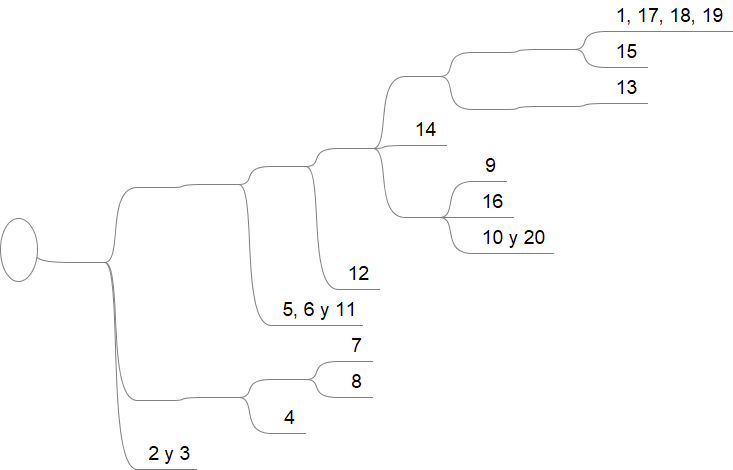
\includegraphics[width=0.8\columnwidth]{CapituloI/Imagenes/Arbol.png}
\caption{Ejemplo del árbol ideal generado al pasar 20 días de uso de una PC.}
\label{fig:arbol}
\end{figure}